\chapter{Teori}\label{Teori}

\section{Trafik Model}

Til dette projekt har vi valgt at arbejde med emnet trafik og simulering, mere specifikt simulering af trafik. Vi agter altså at løse et problem inde for dette område hvor i vores fokus ligger på at lave en simulering der kan hjælpe med til at konstruere og udspille forskellige scenarier der kan udspille sig i traffikerede områder og på den måde også simulerer alternativer. Derfor har gruppen valgt at udarbejde en model der beskriver gruppens fælles definition på trafik. Formålet med dette er at have en model at arbejde med og inddrage i programmet der fungerer som produktet i dette projekt.

OBS: Dette afsnit er ikke færdigt og modellen kan og vil med høj sandsynlighed ændre sig igennem projektet af forskellige årsager! 

\subsection{Trafik Flow}

En publikation fra 1988 af en Paul Ross fra Traffic Systems Division, belyser om emnet Traffic Dynamics og herunder Traffic Flow \cite{trafdyn}. Som Paul Ross beskriver så området et af dem der er mindst forstået da der på dette tidspunkt ikke var nogle kontinuum teorier der kunne forudse trafik densitet, volume og fart med den præcision som der forventes for at kunne opstille et timing signal. Derimod er det bedste der kan gøres er at lave et cirka estimate med diskontinuerlig dellinger. Publikationen forklarer i større detalje hvordan at for at få et udbytte med kontrol, simulation og en general forståelse for emnet, er en beskrivelse af trafik med henhold til fortsættende og differentiable kvantitativer nødvendig. Formålet med denne publikation er at udvikle en ny formulering til dette som er kvalitativt korrekt. 

Den generelle konsensus for trafik variabler er følgende: Trafik Densiteten, k, farten, v, og volume, Q, er passende og brugbare til formået beskrevet herover. Med disse variabler er to relationer kendt. Den første er forbundet i definitionenerne på volume, densitet og fart.

\begin{verbatim}\label{eq:Equation1}
[Q = kv]
\end{verbatim}

\begin{equation}\label{eq:Equation1}
\[Q = kv \]
\begin{flushright}
(1)
\end{flushright}
\end{equation}
						
hvor følgende er gældende:

Q = trafik volume (Bil(er)/timen) forbi et punkt.
k  = vehicular densitet (bil(er)/mi)
v  = (local space-mean) fart (km/t)

Det andet kendte relation, kontinuiteten af fartøjer også nævnt i Paul Ross' rapport \cite{trafdyn}

\begin{equation}\label{eq:Equation2}
\[ \partial k/ \partial t + \partial Q/ \partial x = S(x, t) \]
\begin{flushright}
(2)
\end{flushright}
\end{equation}

Hvor følgende er gældende:
\partial / \partial t+ og \partial / \partial t 
indikerer delvis differentiering i forhold til tiden, t, og lokation på en vej x.
S(x,t) er fartøjer der køre ind på (positive) og køre ud igen (negative) på en vejbane (veh/(km/t)).

Disse to ligninger er dog ikke de eneste der er nødvendige for en fuldendt formulering af trafik flow. En tredje relation er også nødvendigt.

\vspace{5mm}

Der har igennem tiderne været mange bud på hvad denne tredje relation kan være for at få et godt estimat udregnet. Et af disse har været “Deterministic speed-density hypothesis” men Ifølge Paul Ross er dette deterministisk forhold ikke muligt, der er ikke fundet data som bekræfter det på trods af at der er en generel tendens hvorved fart falder jo større trafik densiteten stiger, har ingen observationer der er blevet lavet i dette felt påpeget en bestemt fart til en bestemt densitet.

\vspace{5mm}

En anden relation vil være “Equilibirum Speed-Density Hypothises” som Paul Ross beskriver, denne relation er også blevet beskrevet i en serie af publikationer fra 1961 til og med 1971. Heri beskrives der at trafik har en ligevægts fart distribuering og at det medføre at den aktuelle fart distribuering forsøger at på sin vis “slappe af”. Det er altså underforstået at der er tale om en gennemsnitsfart, men denne relation lider af mange, hvis ikke flere problemer som den sidstnævnte relation, den deterministiske.

\vspace{5mm}

Med dette taget i betragtning kigges der derfor istedet på følgende relation som er formuleret ud fra logiske analyse samt observationer foretaget af Hurdle og Solomon i 1986[5]. Disse indikerer at overbelastning på vejene reducere den ønskede trafik hastighed, men derimod sænker den aktuelle hastighed på vejene mens personer bag rettet har stadig den far de ønsker at rejse i deres free-flow. Relationen kan udtrykkes som følgende:

\begin{equation}\label{Equation 3}
\[ \partial v + v \partial t = (F - v)~T, k < kjam 	\]\begin{flushright}
(3)
\end{flushright}
\end{equation}

Hvor:
F = fri fart på et anlæg (Vejbane) (km/t)
T = “Afslapnings tid” (Timer)
Kjam = “jam” densitet af trafik (vch/km)

F er i denne sammenhæng en konstant som er uafhængig af densiteten, k. Dette vil måske virke ulogisk i lys af observationer der viser at fartøjs trafik bevæger sig langsommere når densiteten er høj. Med de rette afgrænsede forhold vil lining (1), (2), og (3) give et fuldendt afbildning af fart, volume, og densiteten på hvilken som helst plads, x, på hvilket som helst tidspunkt, t. De tre lininger fungerer også således at der ses en opførsel meget lig den man ser i rigtig trafik med “trafik bølger” og livagtigt genoprettelse fra overgangstilstande.

Contraints:

Capacity Limit
De to relationer, den deterministiske og equilibriums relationerne, bliver kapaciteten af vejene bestemt af formed af fart-densitets kurven. Men vores formulering anvender ikke disse to og mangler derfor en lignende begrænsning, derfor formuleres dette på følgende måde for vores model: 

\begin{equation}\label{Equation 4}
\[v ≤ Capacity / k	\]\begin{flushright}
(4)
\end{flushright}
\end{equation}

Denne ulighed fremmer at trafikken vil reducere sin fart således at flowet igennem en indsnævring ikke vil gå ud over kapaciteten af denne indsnævring. Basseret på Paul Ross’s observationer at dette er, kvalitativt, hvad der også sker i rigtige indsnævringer.

Jam density
Med disse ligninger har vi nu en udemneærket repræsentation af trafik ved lave densiteter som også nu fungerer med kapacitet som en form for begrænsning. Dette beskriver dog ikke trafikkens opførsel når trafikkens densitet når sit maksimum, kjam.

\begin{equation}\label{Equation 5}
\[k ≤ k_jam.\]\begin{flushright}
(5)
\end{flushright}
\end{equation}

Som Paul Ross beskriver kjam, så er kjam en konstant som kan ændre sig fra sted til sted, alt efter antallet af vejbaner, men den er ikke afhængig af den fart som trafikken bevæger sig med. Sammenligningen med væsker gør sig gældene igen. En væske’s flow har en volume som er uafhængig af x men dette er ikke inkorporeret i vores formulering endnu. hvis vi tager lign (3) så antages det eksplicit at trafik er komprimerbart. Således kan jam densiteten for lign (4) ændre til følgende.

\begin{equation}\label{Equation 6}
\[  \partial Q/ \partial x = 0, k = k_jam 	\]\begin{flushright}
(6)
\end{flushright}
\end{equation}

Med relationer (1), (2), (3), (4), (5) og (6) har vi nu en komplet formulering af trafik som kan inddrages i vores program.
Note: Nogle dele kan nok godt omformuleres

Lastbiler:
Lastbiler og andre transport fartøjer er oftest skyld i at trafikken går langsommere eller i nogle tilfælde stopper helt op. Det er derfor at bl.a. transport af vindmølledele bliver igangsat sent om aften eller meget tidligt på morgenen således at de ikke skaber problemer for andre billister. Dette har altså en stor effekt på trafikken og kunne derfor være relevant at medtage i vores model, dette er dog ikke gruppens fokus da dette er et meget specifikt scenarie.
NOTE: Kan ændres skulle vi have tid til at lave noget med denne type scenarie.

Tid på dagen / Rush Hour: 
Rush hour er det scenarie hvori der sker mest trafik i et land. Dette er typisk i de timer hvor de forskellige bilister skal på arbejde, køre børn til skole eller andre institutioner eller lignende og igen når disse samme individer skal hjem igen. Dette kan indskrives i programmet som en form for variable der ændre mængden af trafik ved bestemte tidspunkter.
NOTE: Mangler kilde på dansk rush hour.

\section{Dijkstras Algoritme}

Dijkstras algoritme er en algoritme til at finde den korteste vej fra et bestemt punkt til et andet punkt. Disse punkter kan bland andet repræsentere den korteste vej mellem to forskellige byer. Dijkstras er en grådig algoritme, da den finder den korteste længde først og fortsætter således.\cite{DMATBOGEN}

\vspace{5mm}

Dijkstras algoritme finder den korteste rute mellem 2 forskellige punkter i en simpel ikke-orienteret vægtet graf. Man kan se på figur \ref{fig:dijkstrasgraf} at der angives forskellige punkter {A, B, C, D, E, Z}. Hvis man skal fra punkt A til Z på figuren, så starter man ved A og derfor initialiseres A til at være 0, som man kan se på tabel \ref{fig:dijkstratabel}. Algoritmen virker således, at alle punkter er uendeligt udover det punkt man befinder sig på som vist på tabel \ref{fig:dijkstratabel}. Algoritmen tager punkt fra punkt, så den starter med at se de grene som A har. Disse er |AB| = 4 og |AC| = 2. Her fra kan algoritmen ikke se videre end B og C. Den ser altid på det mindste tal, og derfor tager den længden fra A til B som er 4 og længden fra A til C som er 2, begge disse tal er mindre end uendeligt. Herefter ser den efter hvilket af de nuværende tal som er mindst, hvilket er 2. Så derfor vælger den C som sit næste punkt. Algoritmen finder nu de næst tætteste punkt, ved at addere alle de tidligere ruter, som har den korteste rute fra A til det næste sæt af punkter. Her ser algoritmen ud fra C og hvilke grene C har. Dette er længden til B, D og E, dog er længden altid fra A, så derfor er længden fra A til E 12 da 2+10 = 12. Længden til B er nu blivet 3, da algoritmen ser på den korteste rute, så A til B er 3, da 2+1 = 3. Således fortsætter algoritmen indtil den rammer Z.\cite{DMATBOGEN}

\begin{figure}[ht!]
\begin{adjustbox}{width=1.2\textwidth,center=\textwidth}
\centering
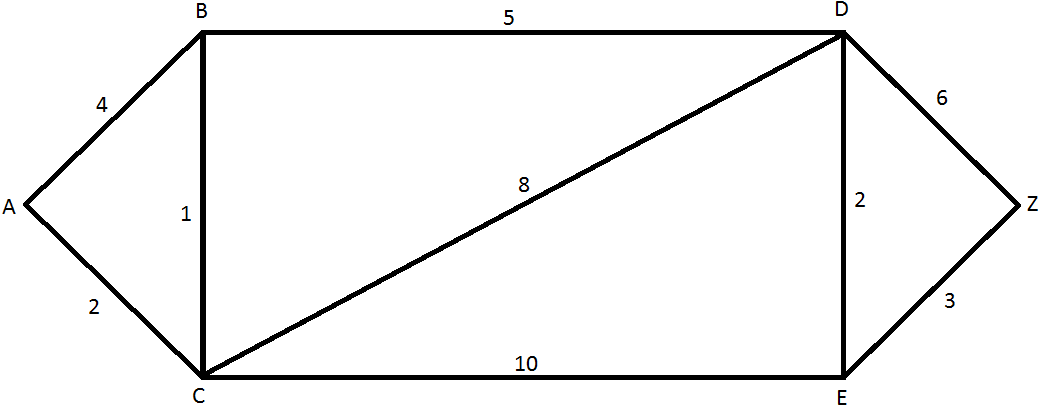
\includegraphics[width=1.2\textwidth]{Pictures/Teoriafsnit/Figurfiler/dijkstrasgraf.png}
\end{adjustbox}
\label{fig:dijkstrasgraf}
\caption{Graf til fremvisning af eksempel af Dijkstras algoritme i brug}
\end{figure}

\begin{table}[ht!]
\centering
\begin{adjustbox}{width=1\textwidth}
\Large
\begin{tabular}{| c | c | c | c | c | c | c |}
	\hline
	 & A & B & C & D & E & Z \\
	\hline
	 & 0 & Inf & Inf & Inf & Inf & Inf \\
	\hline
	{A} & 0 & 4 & 2 & Inf & Inf & Inf \\
	\hline
	{A, C} & 0 & 3 & 2 & 10 & 12 & Inf \\
	\hline
	{A, C, B} & 0 & 3 & 2 & 8 & 12 & Inf \\
	\hline
	{A, C, B, D} & 0 & 3 & 2 & 8 & 10 & 14 \\
	\hline
	{A, C, B, D, E} & 0 & 3 & 2 & 8 & 10 & 13 \\
	\hline
	{A, C, B, D, E, Z} & 0 & 3 & 2 & 8 & 10 & 13 \\
	\hline
\end{tabular}
\end{adjustbox}
\caption{Dijkstra tabel}\label{fig:dijkstratabel}
\end{table}

\begin{lstlisting}[language=C,caption={Dijkstras angivet som eksempel i pseudo-kode},label={lst:DijsktrasPseudo1}]
	procedure Dijkstras(G: weighted connected simple graph, with all weights positive)
{G has vertices a = V0, V1, ....... Vn = z and lengths w(Vi, Vj) where w(Vi,Vj) = infinity if{Vi, Vj} is not an edge in G}
for (i = 1 to n)
	L(Vi) = infinity
L(a) = 0
S = NULL
{ the labels are now initialized so that the label of a is 0 and all other labels are infinity, and S is the empty set }
while (z does not belong to S)
	u = a vertex not in S with L(u) minimal
	S = S U {u}
	for (all vertices v not in S)
		if (L(u) + w(u, v) < L(v) then L(v) = L(u) + L(u, v))
		{this adds a vertex to S with minimal label and updates the labels of vertices not in S}
return (L(z)) {L(z) = length of a shortest path from 	a to z}
\end{lstlisting}

\vspace{5mm}

\section{INTRO TIL TEORI, SKAL SÆTTES I LØSNINGSAFSNIT}
Til udformning af vores løsningsmodel bidrager dette afsnit en gennemang af to algoritmer til ruteplanlægning og vejvisning. De er valgt på baggrund af deres udbredthed i industrien (KILDE). TEKNOLOGIANALYSEN anleder til at afgøre hvilke(n) algoritme(r) der er nødvendige til vores løsningsmodel. Der er blevet valgt to algoritmer til vejvisning som er A* og Dijkstras Algoritme.
Der vil først blive gennengået deres generelle funktion og dernæst en sammenligning af de to og en videre afgrænsning til hvilken der vil blive benyttet til løsningsmodellen.

\vspace{5mm}

\section{A* Algoritmen}
Primært når det kommer til belægning af en dynamisk rute, foregår det ved at en enhed fortsætter hen i mod et mål indtil den når en forhindring. Dette er et ekstremt simpelt bevægelsesmønster og indebærer in vis in-effektivitet. Rent retorisk kunne man stille spørgsmålet om det ikke ville være smartere at planlægge en rute før man overhovedet bevæger sig.

\vspace{5mm}

A* er en algoritme til at beregne den korteste rute baseret på en række heuristiske datasæt. A* får input igennem en brugerlavet graf der indeholder en række datasæt for at algoritmen kan fungere.  Først har vi distancen fra punkt til punkt, eksempelvis punkt 'A' til punkt 'B' som vi kalder for f.eks. \textbf{'H'} og dernæst har vi et datasæt \textbf{'G'} der indeholder bekostningen for at flytte fra en kant til en anden, denne variabel er bestemt på forhånd. Et virkelighedseksempel kunne være at man vil over på den anden side af en sø, så har man så muligheden for at svømme direkte eller gå uden om og det koster f.eks. 2 gange så meget at bevæge sig direkte igennem søen. Dette er givet ved \textbf{'G'}, hvor som sagt \textbf{'H'} er den ultimative korteste længde til det bestemte slutpunkt. \textbf{'H'} fungerer desuden for hvilket som helst punkt i et system og angiver \textit{altid} den korteste vej til slutpunktet uanset forhindringer. Det skal også nævnes at \textbf{'H'} ikke er påvirket af bevægelsesbekostningen, til at starte med, som \textbf{'G'} angiver, dette kommer først senere. Til sidst har vi \textbf{'F'} der er en samenlagt værdi af både \textbf{'H'} og \textbf{'G'}. Dette gælder kun for hver kasse der flyttes til, hvori \textbf{'H'} er angivet ved kassen man flytter tils \textbf{'H'} værdi. Det kan vises således i formlen \ref{eq:A*}:
\begin{equation} \label{eq:A*}
F(n) = G(n) + H(n)
\end{equation}

En måde man kan visualisere A* på er f.eks. med et gitter-system som set i figur \ref{fig:AKvadrat1}. Her kan vi se at vi har et start punkt (grøn) og et slutpunkts (blå). De kasser vi ikke kan bevæge os igennem er de røde kasser. Figuren angiver ingen heuristiske datasæt endnu.

\begin{figure}[ht!]
\begin{adjustbox}{width=1.2\textwidth,center=\textwidth}
\centering
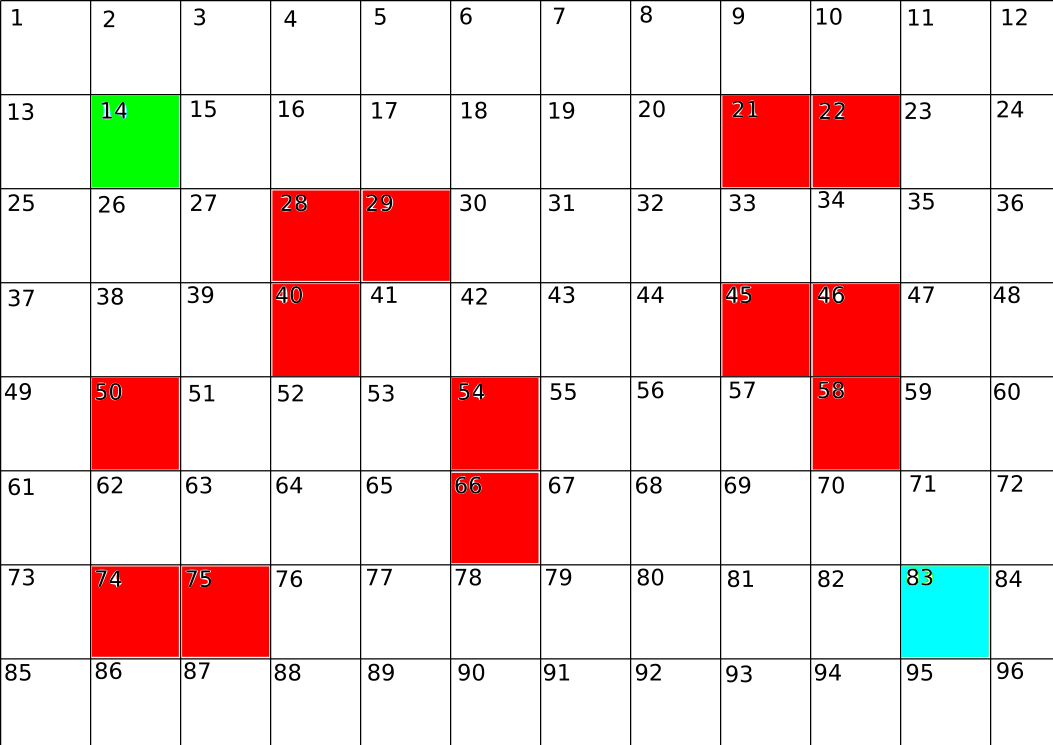
\includegraphics[width=1.2\textwidth]{Pictures/Teoriafsnit/Figurfiler/Grid2.png}
\end{adjustbox}
\label{fig:AKvadrat1}
\caption{A* gitter-system}
\end{figure}

Ud fra figuren kan vi begynde os at forestille hvordan A* fungerer. Når man bevæger sig fra kasse til kasse laver man 2 lister til at holde styr på hvor brikken har været. En liste til at holde styr på hvilke kasser man ikke har besøgt endnu og en liste der holder styr på hvilke man \textbf{har} besøgt. Når man flytter brikken skal man derfor angive hvilken kasse der nu skal på \textit{besøgt} listen. Derfor som nævnt skal vi bruge information om hvor meget \textbf{'G'} koster. Brikken skal nu til at flytte sig for at komme til slutpunktet. Dette kunne f.eks. være 10 point for at flytte sig i hvilken som helst retning, men man kunne også sagtens angive at diagonal bevægelse ville koste 12 point. Dvs. at ruten ændrer sig til måske ikke at være så direkte som den ellers kunne have været.

Der findes flere metoder man kan anvende A* på og en af dem vises her.
Det vises her i den lille bid af Python-kode i Listing \ref{lst:Apseudo1}:
\begin{lstlisting}[caption={A stjerne og pseudo-kode af brug af lister},label={lst:Apseudo1},language=C]
frontier = Queue()
frontier.put(start)
visited = {}
visited[start] = True

while not frontier.empty():
   current = frontier.get()
   for next in graph.neighbors(current):
      if next not in visited:
         frontier.put(next)
         visited[next] = True
\end{lstlisting}
\cite{stanfordredblobgamesAstar}

Som set i figur \ref{fig:AKvadrat1} har vi vores liste givet ved kassernes nummerering. Nummereringen kører fra venstre mod højre én række ad gangen. Vi angiver at det tager 10 point af gå lodret og vandret én kasse ad gangen og 12 point at gå diagonalt. I figur \ref{fig:AKvadrat2} kan vi nu se de heuristiske datasæt angivet fra startpunktet (grøn). Hver enkel kasse omkringliggende startpunktet har deres \textbf{'H'} værdi angivet med lys-lilla tekst og bevægelsesomkostningen \textbf{'G'} fra startpunktet til kassen angivet i blå tekst.

\begin{figure}[ht!]
\begin{center}
\includegraphics[width=1.00\textwidth]{Pictures/Teoriafsnit/Figurfiler/Grid3.png}
\end{center}
\label{fig:AKvadrat2}
\caption{A* der viser bekostning af bevægelse fra startpunkt (grøn) til omkringliggende kasser ('G') angivet med blå farve samt 'H' angivet med lys-lilla}
\end{figure}

Nu udregnes \textbf{'F'} værdien så f.eks. hvis vi går fra kasse 14 (startpunktet) til 15 skal vi lægge 10 (\textbf{'G'}) og 8 (\textbf{'H'}) sammen. Dette gør vi så for alle omkringliggende kasser for startpunktet. Dernæst går man til den laveste \textbf{'F'} værdi og gør helt det samme som før, derudover flyttes den nye kasse man står på til \textit{besøgt} listen. Noget man skal være opmærksom på her er at man stadig skal sammenligne bevægelsesomkostningen fra den tidligere kasse til de kasser der også er relevante for den nye kasse man har flyttet sig til. For dermed at afgøre om man kunne have påført en smartere bevægelse.

Denne fremgangsmåde er også bedre kendt som Breadth First Search, hvori en frontlinje bliver kontinuerligt fremskyndet baseret på omkostninger og heuristiske datasæt\cite{stanfordredblobgamesAstar}.
A* er en heuristisk fremgangsmåde afledt af Dijkstras generelle funktionalitet. %\cite{http://search.proquest.com/openview/88fa950a98b308c6687f79f76caeb187/1?pq-origsite=gscholar}


\subsection{Dijkstra og A* sammenligning}
